
\documentclass[a4paper,14pt]{extarticle}

\usepackage{pythontex}

% for ability to highlight\select and copy text from result pdf output to
% clipboard
\usepackage{cmap}

\usepackage{comment}

\usepackage{setspace}

\usepackage[labelsep=period]{caption}

\usepackage{graphicx}
\graphicspath{ {figure/} }

\usepackage{float}

\usepackage[T2A]{fontenc}
\usepackage[utf8]{inputenc}
\usepackage[russian]{babel}

\usepackage[a4paper,margin=1cm,footskip=1cm,left=2cm,right=1.5cm,top=1.5cm,
		bottom=2cm]{geometry}

\usepackage{textcase}
\usepackage{csquotes}
\usepackage{enumitem}

\usepackage[nottoc]{tocbibind}

% do not show section numbers
%\usepackage[raggedright]{titlesec}

\usepackage{amsmath}

% indent first paragraph in every section
\usepackage{indentfirst}

\usepackage{secdot}

\usepackage[titletoc,title]{appendix}


% indent description items
\setlist[description]{leftmargin=\parindent,labelindent=\parindent}

% ?
%\patchcmd{\appendices}{\quad}{: }{}{}

\setcounter{secnumdepth}{3}
\setstretch{1.5}

\DeclareMathOperator{\Sp}{Sp}

\let\oldref\ref
\renewcommand{\ref}[1]{(\oldref{#1})}

\begin{document}

\begin{comment}
\begin{titlepage}

	\begin{center}
		\MakeTextUppercase{Министерство образования и науки Российской~Федерации}

		\bigbreak

		ФЕДЕРАЛЬНОЕ ГОСУДАРСТВЕННОЕ БЮДЖЕТНОЕ ОБРАЗОВАТЕЛЬНОЕ УЧРЕЖДЕНИЕ
			ВЫСШЕГО ОБРАЗОВАНИЯ

		\bigbreak

		\MakeTextUppercase{\enquote{Новосибирский государственный технический
			университет}}
		\vspace{5pt}
		\hrule

		\bigbreak

		Кафедра теоретической и прикладной информатики

		\vspace{50pt}

		\textbf{\LARGE{Отчет по}\\}

		\bigbreak

		производственной практике: \\
			практике по получению профессиональных умений и опыта профессиональной
			деятельности

		\bigbreak

		c 1 ноября по 31 декабря

		\bigbreak

		<<Параметрическая идентификация стохастических динамических линейных
		непрерывно-дискретных систем>>

		\vspace{50pt}

	\end{center}

	\begin{flushleft}
		\begin{tabbing}
			Группа:\qquad\qquad\qquad \= ПММ-61\\
			Студент:                  \> Горбунов К. К.\\
			Место практики:           \> отдел № 8 ФГУП <<СНИИМ>> \\
			Руководитель:             \> нач. отдела № 8, Толстиков А.С.
		\end{tabbing}
	\end{flushleft}

	\begin{center}
		\vspace{\fill}
		Новосибирск, 2016 г.
	\end{center}

\end{titlepage}
\end{comment}

\tableofcontents

\newpage

\section*{Введение}
\addcontentsline{toc}{section}{Введение}

В настоящее время математическое моделирование играет фундаментальную роль в
науке и технике и является одним из интенсивно развивающихся перспективных
научных направлений в области информатики.

Проблема идентификации, связанная с построением математических моделей по
экспериментальным данным, относится к одной из основных проблем теории и
практики автоматического управления. Ее качественное решение способствует
эффективному применению на практике современных математических методов и
наукоемких технологий, например, при расчете и проектировании систем управления
подвижными (в том числе авиационно-космическими) и технологическими объектами,
построении прогнозирующих моделей (например, в экономике и бизнес-процессах),
конструировании следящих и измерительных систем \cite{denisov}.

\section{Постановка задачи}

\subsection[Структурно-вероятностное описание модельной структуры]
{Структурно-вероятностное описание модельной \\структуры}

\renewcommand{\vec}[1]{\mathbf{#1}}

Определим модель стохастической динамической линейной \\непрерывно-дискретной
системы в простанстве состояний в общем виде:
\begin{equation}
	\label{eq:initmod}
	\left\{ 
		\begin{array}{lll}
			\frac{d}{dt}\vec{x}(t) &= F \vec{x}(t) + C \vec{u}(t) + G
				\vec{w}(t), & t \in [t_0,T] \\ 
			\vec{y}(t_k)           &= H \vec{x}(t_k) + \vec{v}(t_k), 
				& k = 1,\ldots, N
		\end{array} 
	\right. 
\end{equation}

Здесь:
\begin{description}
  \item [$\vec{x}(t)$] -- $n$-вектор состояния;
  \item [$F$] -- матрица перехода состояния;
  \item [$\vec{u}(t)$] -- $r$-вектор управления (входного воздействия);
  \item [$C$] -- матрица управления;
  \item [$\vec{w}(t)$] -- $p$-вектор возмущений;
  \item [$G$] -- матрица влияния возмущений;
  \item [$H$] -- матрица наблюдения;
  \item [$\vec{v}(t_{k+1})$] -- $m$-вектор шума измерений;
  \item [$\vec{y}(t_{k+1})$] -- $m$-вектор наблюдений (измерений) отклика;
\end{description}

$F, C, G, H$ --- матрицы соответствующих размеров.

\bigskip
Априорные предположения:
\begin{itemize}
\item $F$ устойчива;
\item пары $(F, C)$ и $(F, G)$ управляемы;
\item пара $(F, H)$ --- наблюдаема;
\item случайные процессы $\{\vec{w}(t), t \in [t_0, T]\}$ и
	$\{\vec{v}(t_{k}), k = 1, 2, \ldots, N\}$ являются стационарными белыми
		гауссовскими шумами, причем:
\[
	E[\vec{w}(t)] = 0,\ E[\vec{w}(t)\vec{w}^{T}(\tau)] = Q \delta(t-\tau)\,
\]
\[
	E[\vec{v}(t_k)] = 0,\ E[\vec{v}(t_k)\vec{v}^{T}(t_j)] = R \delta_{k,j}\,
\]
\[
	E[\vec{v}(t_k)\vec{w}^{T}(t)] = 0,\qquad \forall t_k, t,
\]
		где $\delta(t-\tau)$ --- дельта-функция Дирака, $\delta_{jk}$ --- символ
		Кронекера;

\item начальное состояние $\vec{x}(t_0)$ имеет нормальное распределение с
параметрами $\overline{\vec{x}}(t_0)$ и $P(t_0)$ и не коррелирует с
		$\vec{w(t)}$ и $\vec{v_k}$ при любых значениях $t$ и $k$.

Будем считать, что подлежащие оцениванию параметры $\theta = (\theta_1,
\theta_2, \ldots, \theta_s)$ могут входить в элементы матриц $F, C, G, H, Q, R,
P(t_0)$ и в вектор $\overline{\vec{x}}(t_0)$ в различных комбинациях.

\end{itemize}

В данной модели уравнение объекта является непрерывным, а уравнение наблюдений
--- дискретным. Такая модель является характерной для значительного множества
прикладных задач.

Одной из целей исспедований в рамках магистерской диссертации является
разработка алгоритмов оценивания состояния и идентификации стохастической 
динамической непрерывно-дискретной модели вида \ref{eq:initmod}. 

Один из видимых путей решения задачи оценивания состояния такой системы
является адаптация аналогичных алгоритмов, применимых к дискретным и
непрерывным системам, к данному непрерывно-дискретному случаю.

Разрабатываемый алгоритм также должен оценивать вероятностные характеристики
шумов объекта и измерений, потому как в реальных задачах вероятностные
характеристики данных процессов неизвестны или же эти процессы являются
нестационарными.

\section[Параметрическая идентификация моделей стохастических
\\непрерывно-дискретных систем]
{Параметрическая идентификация моделей \\стохастических
непрерывно-дискретных систем} 

Идентификацией динамической системы называется определение структуры и
параметров математической модели, обеспечивающих наилучшее совпадение выходных
переменных моделей переменных модели и системы при одинаковых входных
воздействиях \cite{chubich}.

Под параметрической идентификацией, в частности, понимается только определение
параметров модели. Предполагается, что структура модели известна.

В данной работе в качестве критерия идентификации используется критерий
максимального правдоподобия, а получаемые оценки параметров модели является
оценками максимального правдоподобия (ОМП).

\subsection{Вычисление значения критерия идентификации}

\newcommand{\eps}{\varepsilon}

Выражение для критерия максимального правдоподобия имеет вид \cite{denisov}:
\begin{equation}
\begin{split}
\chi(\theta) = -\ln{L(Y_1^N;\theta)} = \frac{Nm}{2} \ln{2\pi} +
\\ + \frac{1}{2} \sum\limits_{k=1}^{N} 
\left[ \eps^T(t_k, \theta) B^{-1}(t_k, \theta) \eps(t_k, \theta) + 
\ln \det B(t_k, \theta) \right].
\end{split}
\end{equation}

Здесь:

\begin{description}
\item[$Y_1^N$] --- множество из $N$ наблюдений отклика
\item[$\theta$] --- вектор параметров модели 
\item[$\chi(\cdot)$] --- функционал, используемый в качестве критерия
идентификации
\item[$L(\cdot)$] --- функционал максимального правдоподобия 
\item[$N$] --- число дискретных моментов времени наблюдений
\item[$m$] --- число выходных каналов системы (размерность вектора наблюдений
отклика)
\item[$\eps(t_j) = y(t_j) - H \hat{x}(t_j|t_{j-1})$] --- обновляющая
последовательность 
\item[$B(t_j) = HP(t_j|t_{j-1})H^T + R$] --- ковариационная обновляющей
последовательности 
\end{description}

\newpage
Алгоритм вычисления значения критерия следующий:

\begin{enumerate}
\item Пусть $j = 1$, $\chi(\theta) = 0$.
\item Решаются дифференциальные уравнения непрерывно-дискретного фильтра
Калмана с соответствующими начальными условиями:
\[
\frac{d}{dt}\hat{x}(t|t_{j-1}) = F \hat{x}(t|t_{j-1}) + C u(t),\ 
t_{j-1} \le t \le t_j,\ \hat{x}(t_0|t_0) = \bar{x}_0;
\]
\[
\frac{d}{dt}P(t_j|t_{j-1}) = F P(t|t_{j-1}) + P(t|t_{j-1}) F^T + GQG^T,\\
\]
\[
t_{j-1} \le t \le t_j,\ P(t_0|t_0) = P_0;
\]
Получаем $\hat{x}(t_j|t_{j-1})$ и $P(t_j|t_{j-1})$.

\item Вычисляются
\[ \eps(t_j) = y(t_j) - H \hat{x}(t_j|t_{j-1}); \]
\[ B(t_j) = H P(t_j|t_{j-1}) H^T + R; \]
\[
K(t_j) = P(t_j|t_{j-1}) H^T B^{-1}(t_j).
\]

\item Вычисляется соответствующая $j$-му моменту времени составляющая функции
правдоподобия (2.35)
\[
S = \frac{1}{2} \left[ B^{-1}(t_j) \eps(t_j) + \ln \det B(t_j) \right].
\]

\item Накапливается сумма
\[
\chi(\theta) = \chi(\theta) + S.
\]

\item Если $j = N$, то
\[
\chi(\theta) = \chi(\theta) + \frac{Nm}{2} \ln 2\pi
\]
и вычисления прекращаются, иначе --- вычисляются следующие начальные условия по
формулам
\[
\hat{x}(t_j|t_{j-1}) = \hat{x}(t_j|t_{j-1}) + K(t_j) \eps(t_j);
\]
\[
P(t_j|t_{j-1}) = \left[ I - K(t_j) H \right] P(t_j|t_{j-1}),
\]
$j$ заменяется на $j+1$ и осуществляется переход на шаг 2.

\end{enumerate}

\subsection[Вычисление значения градиента критерия идентификации]
{Вычисление значения градиента критерия \\идентификации}

В данной работе предлагается к рассмотрению два практических метода вычисления
значения градиента критерия идентификации: по аналитическому выражению и с
использованием программных средств автоматического дифференцирования.

Далее приведено краткое описание каждого из этих методов.

\subsubsection{Вычисление по аналитическому выражению}


Аналитическое выражение производных критерия следующее \cite{denisov}:

\begin{multline}
	\label{eq:llderiv}
	\frac{\partial \chi(\theta)}{\partial \theta_k} = \sum\limits^{N}_{j=1}
	\left[
	\eps^{T}(t_j) B^{-1}(t_j) \frac{\partial \eps(t_j)}{\partial \theta_k} -
	\frac{1}{2} \eps^{T}(t_j) B^{-1}(t_j) \frac{\partial B(t_j)}
	{\partial \theta_k}
	B^{-1}(t_j) \eps(t_j) + \right.\\\left.
	\frac{1}{2}
	\Sp \left( B^{-1}(t_j) \frac{\partial B(t_j)}{\partial \theta_k} \right)
	\right] ,\ k = 1,\ldots,s,
\end{multline}
где $s$ --- размерность вектора неизвестных параметров $\Theta$.

В выражении \ref{eq:llderiv} частные производные $\frac{\partial \eps(t_j)}
{\partial \theta_k}$ и $\frac{\partial B(t_j)}{\partial \theta_k}$ вычисляются
с помощью следующим выражений:
\begin{equation}
\frac{\partial \eps(t_j)}{\partial \theta_k} = - \frac{\partial H}
{\partial \theta_k} \hat{x}(t_j|t_{j-1}) - H \frac{\partial 
	\hat{x}(t_j|t_{j-1})}
{\partial \theta_k},\\
\end{equation}

\begin{equation}
\frac{\partial B(t_j)}{\partial \theta_k} = \frac{\partial H}
	{\partial \theta_k}
P(t_j|t_{j-1}) H^T + H \frac{\partial P(t_j|t_{j-1})}{\partial \theta_k} H^T +
H P(t_j|t_{j-1}) \frac{\partial H^T}{\partial \theta_k} + \frac{\partial R}
{\partial \theta_k}.
\end{equation}

Уравнения чувствительности для оценки вектора состояний:
\begin{multline}
\label{eq:senstate}
\frac{d}{dt}
\begin{bmatrix}
	\hat{x}(t|t_{j-1}) \\
	\frac{\partial \hat{x}(t|t_{j-1})}{\partial \theta_1} \\
	\vdots \\
	\frac{\partial \hat{x}(t|t_{j-1})}{\partial \theta_s}
\end{bmatrix} =
\begin{bmatrix}
	F \hat{x}(t|t_{j-1}) + G u(t) \\
	\frac{\partial F}{\partial \theta_1} \hat{x}(t|t_{j-1}) +
		F \frac{\partial \hat{x}(t|t_{j-1})}{\partial \theta_1} +
		\frac{\partial G}{\partial \theta_1} u(t) \\
	\vdots  \\
	\frac{\partial F}{\partial \theta_s} \hat{x}(t|t_{j-1}) +
		F \frac{\partial \hat{x}(t|t_{j-1})}{\partial \theta_s} +
		\frac{\partial G}{\partial \theta_s} u(t)
\end{bmatrix} = \\ =
\begin{bmatrix}
	F & 0 & \cdots & 0 \\
	\frac{\partial F}{\partial \theta_1} & F & \cdots & 0 \\
	\vdots & \vdots & \ddots & \vdots \\
	\frac{\partial F}{\partial \theta_s} & 0 & \cdots & F
\end{bmatrix} \cdot
\begin{bmatrix}
	\hat{x}(t|t_{j-1}) \\
	\frac{\partial \hat{x}(t|t_{j-1})}{\partial \theta_1} \\
	\vdots \\
	\frac{\partial \hat{x}(t|t_{j-1})}{\partial \theta_s} \\
\end{bmatrix} +
\begin{bmatrix}
	G \\
	\frac{\partial{G}}{\partial \theta_1} \\
	\vdots \\
	\frac{\partial{G}}{\partial \theta_s}
\end{bmatrix} u(t),\\
\hspace{\fill} t_{j-1} \le t \le t_j,\ j=1,\ldots,N. \hspace{\fill}
\end{multline}

Начальные условия:
\begin{itemize}

\item для $j = 1$

\begin{equation}
\label{eq:senstateinitcond1}
\begin{bmatrix}
	\hat{x}(t_0|t_0) \\
	\frac{\partial \hat{x}(t_0|t_0)}{\partial \theta_1} \\
	\vdots \\
	\frac{\partial \hat{x}(t_0|t_0)}{\partial \theta_s}
\end{bmatrix} =
\begin{bmatrix}
	\overline{x_0} \\
	\frac{\partial \overline{x_0}}{\partial \theta_1} \\
	\vdots \\
	\frac{\partial \overline{x_0}}{\partial \theta_s}
\end{bmatrix}
\end{equation}

\item для $j = 2, 3, \ldots, N$

\begin{equation}
\label{eq:senstateinitcondj}
\begin{bmatrix}
	\hat{x}(t_j|t_j) \\
	\frac{\partial \hat{x}(t_j|t_j)}{\partial \theta_1} \\
	\vdots \\
	\frac{\partial \hat{x}(t_j|t_j)}{\partial \theta_s}
\end{bmatrix} =
\begin{bmatrix}
	\hat{x}(t_j|t_{j-1}) + K(t_j) \eps(t_j) \\
	\frac{\partial \hat{x}(t_j|t_{j-1})}{\partial \theta_1} + 
	\frac{\partial K(t_j)}
		{\partial \theta_1} \eps(t_j) + K(t_j) \frac{\partial \eps(t_j)}
		{\partial \theta_1} \\
		\vdots \\
	\frac{\partial \hat{x}(t_j|t_{j-1})}{\partial \theta_s} + 
	\frac{\partial K(t_j)}
		{\partial \theta_s} \eps(t_j) + K(t_j) \frac{\partial \eps(t_j)}
		{\partial \theta_s}
\end{bmatrix}.
\end{equation}

\end{itemize}

Уравнения чувствительности для ковариационной матрицы оценки вектора состояний:
\begin{multline}
	\label{eq:senscov}
	\frac{d}{dt}
	\begin{bmatrix}
		P(t|t_{j-1}) \\
		\frac{\partial P(t|t_{j-1})}{\partial \theta_1} \\
		\vdots \\
		\frac{\partial P(t|t_{j-1})}{\partial \theta_s}
	\end{bmatrix} = \\
	= \begin{bmatrix}
		F P(t|t_{j-1}) + P(t|t_{j-1}) F^T + G Q G^T \\
		\frac{\partial F}{\partial \theta_1} P(t|t_{j-1}) +
			F \frac{\partial P(t|t_{j-1})}{\partial \theta_1} +
			\frac{\partial P(t|t_{j-1})}{\partial \theta_1} F^T + \hspace{\fill} \\
			\hspace{8em} + P(t|t_{j-1}) \frac{\partial F^T}{\partial \theta_1} +
			\frac{\partial G}{\partial \theta_1} Q G^T +
			G \frac{\partial Q}{\partial \theta_1} G^T +
			G Q \frac{\partial G^T}{\partial \theta_1} \\
		\vdots \\
		\frac{\partial F}{\partial \theta_s} P(t|t_{j-1}) +
			F \frac{\partial P(t|t_{j-1})}{\partial \theta_s} +
			\frac{\partial P(t|t_{j-1})}{\partial \theta_s} F^T + \hspace{\fill} \\
			\hspace{8em} + P(t|t_{j-1}) \frac{\partial F^T}{\partial \theta_s} +
			\frac{\partial G}{\partial \theta_s} Q G^T +
			G \frac{\partial Q}{\partial \theta_s} G^T +
			G Q \frac{\partial G^T}{\partial \theta_s}
	\end{bmatrix}  = \\
	= \begin{bmatrix}
		F & 0 & \cdots & 0 \\
		\frac{\partial F}{\partial \theta_1} & F & \cdots & 0 \\
		\vdots & \vdots & \ddots & \vdots \\
		\frac{\partial F}{\partial \theta_s} & 0 & \cdots & F \\
	\end{bmatrix}
	\begin{bmatrix}
		P(t|t_{j-1}) \\
		\frac{\partial P(t|t_{j-1})}{\partial \theta_1} \\
		\vdots \\
		\frac{\partial P(t|t_{j-1})}{\partial \theta_s}
	\end{bmatrix} +
	\begin{bmatrix}
	P(t|t_{j-1}) & 0 & \cdots & 0 \\
	\frac{\partial P(t|t_{j-1})}{\partial \theta_1} & P(t|t_{j-1}) & \cdots & 0 \\
	\vdots & \vdots & \ddots & \vdots \\
	\frac{\partial P(t|t_{j-1})}{\partial \theta_s} & 0 & \cdots & P(t|t_{j-1})
	\end{bmatrix}
	\begin{bmatrix}
		F^T \\
		\frac{\partial F^T}{\partial \theta_1} \\
		\vdots \\
		\frac{\partial F^T}{\partial \theta_s}
	\end{bmatrix} + \\
	+ \begin{bmatrix}
		G Q G^T\\
		\frac{\partial G}{\partial \theta_1} Q G^T \\
		\vdots \\
		\frac{\partial G}{\partial \theta_s} Q G^T
	\end{bmatrix} +
	\begin{bmatrix}
		0 \\
		G \frac{\partial Q}{\partial \theta_1} G^T \\
		\vdots \\
		G \frac{\partial Q}{\partial \theta_s} G^T
	\end{bmatrix} +
	\begin{bmatrix}
		0 \\
		G Q \frac{\partial G^T}{\partial \theta_1} \\
		\vdots \\
		G Q \frac{\partial G^T}{\partial \theta_s}
	\end{bmatrix},\\ \hspace{\fill} t_{j-1} \le t \le t_j, \quad j = 1, \ldots, N. \hspace{\fill}
\end{multline}

\newpage
Начальные условия:
\begin{itemize}

	\item для $j = 1$

\begin{equation}
\label{eq:senscovinitcond1}
\begin{bmatrix}
	P(t_0|t_0) \\
	\frac{\partial P(t_0|t_0)}{\partial \theta_1} \\
	\vdots \\
	\frac{\partial P(t_0|t_0)}{\partial \theta_s}
\end{bmatrix} =
\begin{bmatrix}
	P_0 \\
	\frac{\partial P_0}{\partial \theta_1} \\
	\vdots \\
	\frac{\partial P_0}{\partial \theta_s}
\end{bmatrix}
\end{equation}

\item для $j = 2, 3, \ldots, N$

\begin{multline}
\label{eq:senscovinitcondj}
\begin{bmatrix}
	P(t|t_j) \\
	\frac{\partial P(t_j|t_j)}{\partial \theta_1} \\
 	\vdots \\
	\frac{\partial P(t_j|t_j)}{\partial \theta_s}
\end{bmatrix} =
\begin{bmatrix}
	\left\{ I - K(t_j) H \right\} P(t_j|t_{j-1}) \\
	\left[ - \frac{\partial K(t_j)}{\partial \theta_1} H - K(t_j)
		\frac{\partial H}{\partial \theta_1} \right] P(t_j|t_{j-1}) + 
		\left\{ I - K(t_j) H \right\}
		\frac{\partial P(t_j|t_{j-1})}{\partial \theta_1} \\
	\vdots \\
	\left[ - \frac{\partial K(t_j)}{\partial \theta_s} H - K(t_j)
		\frac{\partial H}{\partial \theta_s} \right] P(t_j|t_{j-1}) + 
		\left\{ I - K(t_j) H \right\}
		\frac{\partial P(t_j|t_{j-1})}{\partial \theta_s} \\
\end{bmatrix},
\end{multline}

\end{itemize}

где
\begin{multline}
	\frac{\partial K(t_j)}{\partial \theta_k} =
		\frac{\partial P(t_j|t_{j-1})}{\partial \theta_k} H^T B^{-1}(t_j) + 
		P(t_j|t_{j-1}) \frac{\partial H^T}{\partial \theta_k} B^{-1}(t_j) - \\ -
		P(t_j|t{j-1}) H^{-1} B^{-1}(t_j) \frac{\partial B(t_j)}{\partial \theta_k}
		B^{-1}(t_j).
\end{multline}

Алгоритм может быть следующим:

\begin{enumerate} 

\item $j = 1$,\enskip $\frac{\partial \chi (\theta)}{\partial \theta_k} = 0$,
 \enskip $k = 1, \ldots, s$,\quad где $s$ --- размерность вектора \\ параметров
 $\Theta$.

\item Решаются уравнения чувствительности для оценки вектора состояния
\ref{eq:senstate} и его ковариационной матрицы \ref{eq:senscov} с начальными
условиями \ref{eq:senstateinitcond1} и \ref{eq:senscovinitcond1}
соответственно. Получаем $\hat{x}(t_j|t_{j-1})$ и $P(t_j|t_{j-1})$.

\item Вычисляются
\[
	B(t_j) = H P(t_j|t_{j-1}) H^T + R;
\]
\begin{multline}
	\frac{\partial B(t_j)}{\partial \theta_k} =
		\frac{\partial H}{\partial \theta_k} P(t_j|t_{j-1}) H^T + H
		\frac{\partial P(t_j|t_{j-1})}{\theta_k} H^T + \\ +
		H P(t_j|t_{j-1}) \frac{\partial H^T}{\partial \theta_k} +
		\frac{\partial R}{\partial \theta_k},\qquad k = 1, \ldots, s.
\end{multline}

\newcommand{\pd}[2]{\frac{\partial #1}{\partial #2}}

\item Вычисляются
\[
	K(t_j) = P(t_j|t_{j-1}) H^T B^{-1}(t_j);
\]
\begin{multline}
	\pd{K(t_k)}{\theta_i} = \pd{P(t_k|t_{k-1})}{\theta_i} H^T B^{-1}(t_k) +
	P(t_k|t_{k-1}) \pd{H^T}{\theta_i} B^{-1}(t_k) - \\
	- P(t_k|t_{k-1}) H^T B^{-1}(t_k)
	\pd{B(t_k)}{\theta_i} B^{-1}(t_k),\qquad i = 1, \ldots, s.
\end{multline}

\item Вычисляются
\[
	\eps(t_j) = y(t_j) - H \hat{x}(t_j|t_{j-1});
\]
\[
	\pd{\eps(t_j)}{\theta_k} = - \pd{H}{\theta_k} \hat{x}(t_j|t_{j-1}) -
		H \pd{\hat{x}(t_j|t_{j-1})}{\theta_k},\qquad k = 1, \ldots, s.
\]

\item Вычисляется соответствующая $j$-му моменту времени составляющая градиента
функции правдоподобия \ref{eq:llderiv}
\begin{multline}
	S(k) = \eps^T(t_j) B^{-1}(t_j) \pd{\eps(t_j)}{\theta_k} - \frac{1}{2}
	\eps^T(t_j) B^{-1}(t_j) \pd{B(t_j)}{\theta_k} B^{-1}(t_j) \eps(t_j) + \\ +
	\frac{1}{2} \Sp{ B^{-1}(t_j) \pd{B(t_j)}{\theta_k} },\qquad k = 1, \ldots, s.
\end{multline}

\item Накапливается сумма
\[
	\pd{\chi(\theta)}{\theta_k} = \pd{\chi(\theta)}{\theta_k} + S(k),
		\qquad k = 1, \ldots, s.
\]

\item Если $j = N$, то вычисления прекращаются, иначе --- вычисляются следующие
начальные условия по формулам \ref{eq:senstateinitcondj} и
\ref{eq:senscovinitcondj}, $j$ заменяется на $j + 1$, и осуществляется переход
на шаг 2.

\end{enumerate}

\subsubsection{Программный метод автоматического дифференцирования}

Рассматриваемый программный метод берет свое начало из задач машинного обучения
глубоких нейронных сетей, которые в настоящее время являются популярным
объектом научных исследований, образующие целое новое научное направление ---
глубинное обучение (deep learning). Глубокие нейронные сети применяются для
решения широкого класса практических задач распознавания, классификации,
предсказания, обработки и анализа ествесственных языков и многих других.

Глубокими нейронными сетями называются такие сети, которые имеют в своем
составе большое число скрытых слоев нейронов, и, следовательно, суммарно
большое число нейронов.

Задачу обучения нейронной сети можно трактовать как оценивание параметров этой
сети по некоторым полученным извне наборам данных (наблюдениям), которые
называются обучающими наборами данными. Параметрами сети являются веса связей
между её нейронами. Так как по определению глубокой сети число входящих в неё
нейронов велико, то, соответственно, велико и число <<оцениваемых>> параметров
(весов).

В связи с большим числом параметров (весов) возникают проблемы применимости
методов оценивания с использованием традиционных методов вычисления градиента
функции потерь (критерия) для поиска экстремальных значений. Эти проблемы,
связаны, во-первых, с невозможностью вывода аналитического выражения градиента
для модели со столь большим числом параметров (сотни тысяч, миллионы параметров
/ весов) и столь сложной структурой как нейронная сеть. Во-вторых, методы
приближенного вычисления градиента не позволяют достичь удовлетворительной
точности для обеспечения сходимости оптимизационной процедуры к искомому
решению.

Программный метод автоматического дифференцирования или также называемый метод
обратного распространения ошибки основан на правиле дифференцирования сложной
функции --- <<правиле цепи>> (<<chain rule>>), и предполагает определения
производной для каждой операции используемой системы компьютерной алгебры.
Данный метод позволяет вычислять градиент быстро и точно, не программируя явно
его вычисления. Отсюда и название метода --- автоматическое дифференцирование.
Следует отметить, очевидно, что с помощью этого метода также можно вычислять
и производные высших порядков быстро и без потери точности.

\begin{figure}[H]
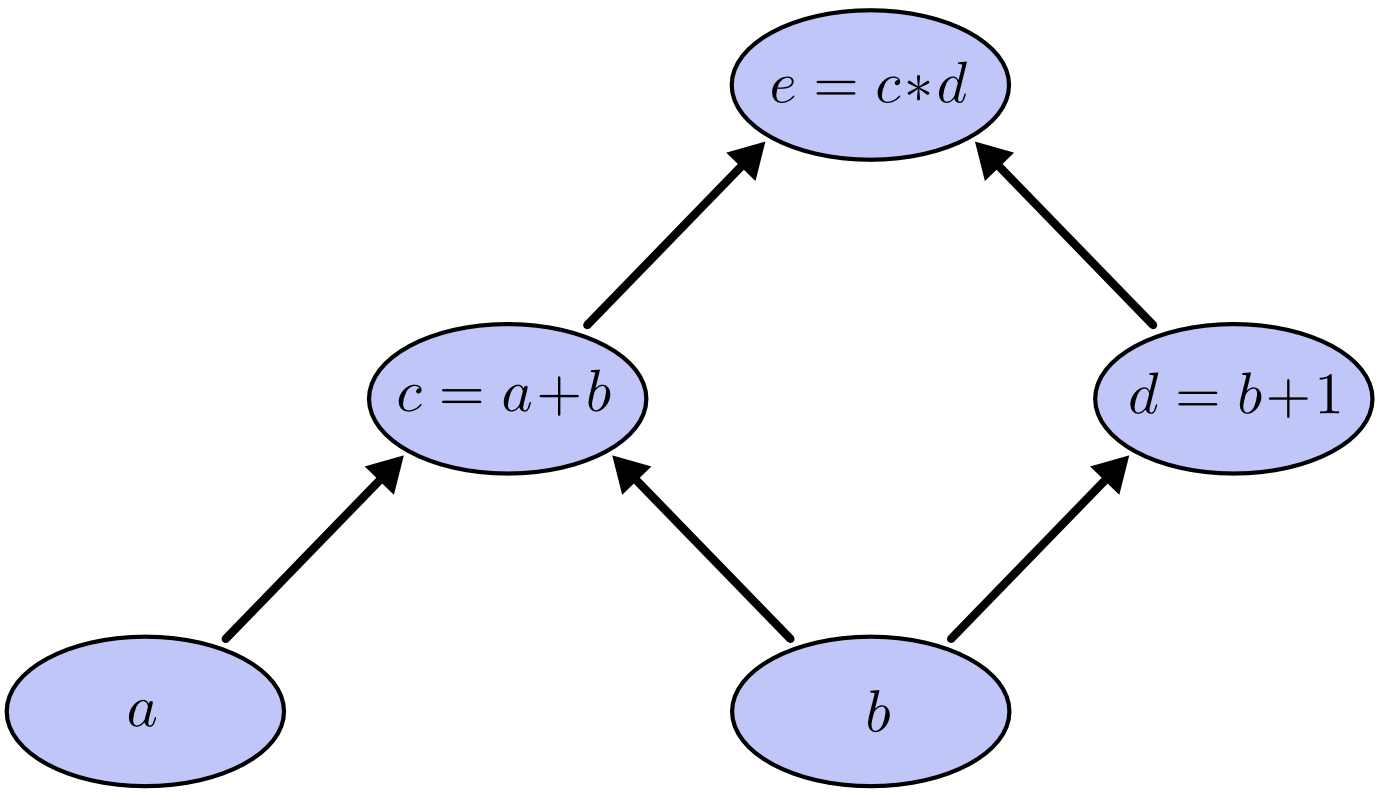
\includegraphics[width=\textwidth]{tree-def}
\caption{Простой пример вычислительного графа \cite{colah}.}
\end{figure}

\begin{figure}[H]
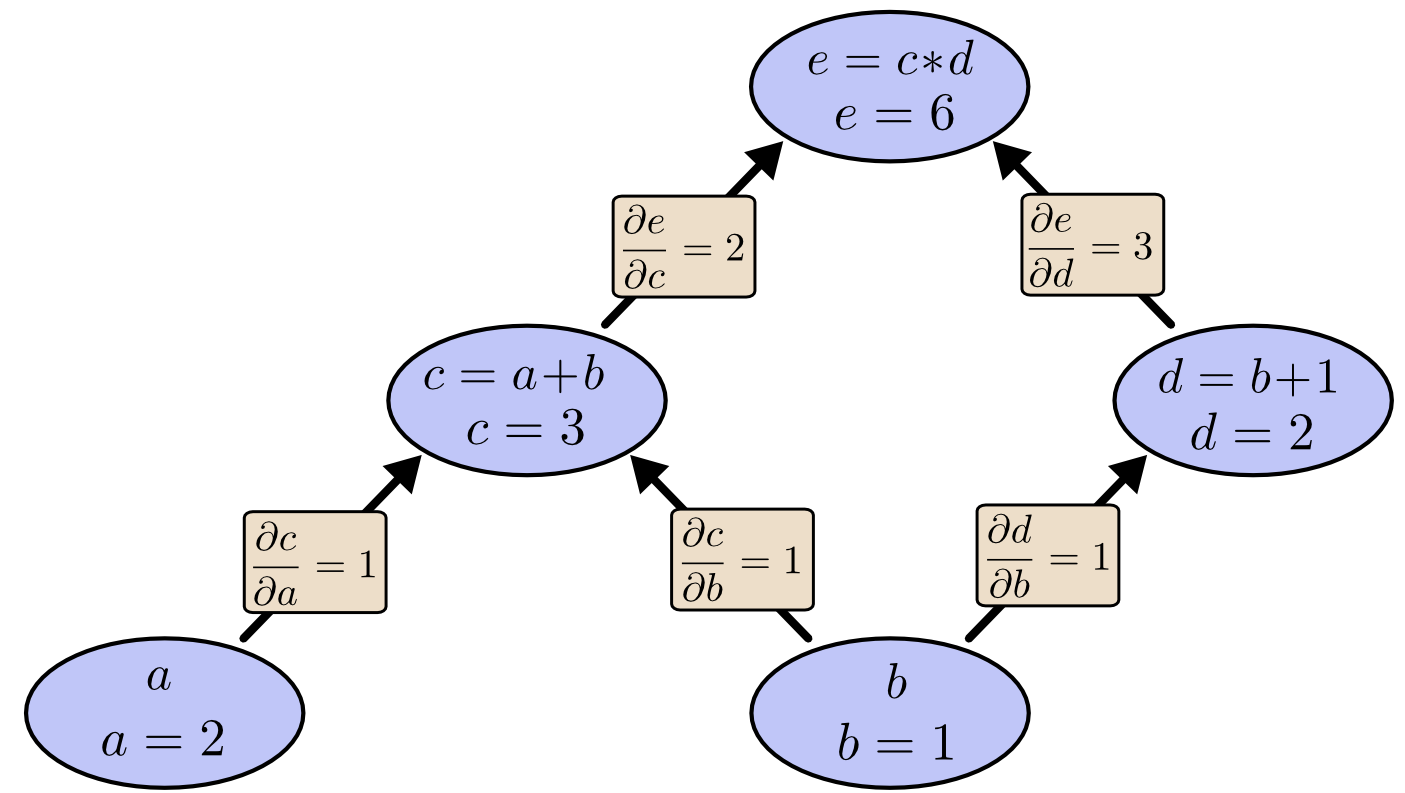
\includegraphics[width=\textwidth]{tree-eval-derivs}
\caption{Пример вычислительного графа с определением производных \cite{colah}.}
\end{figure}

\begin{figure}[H]
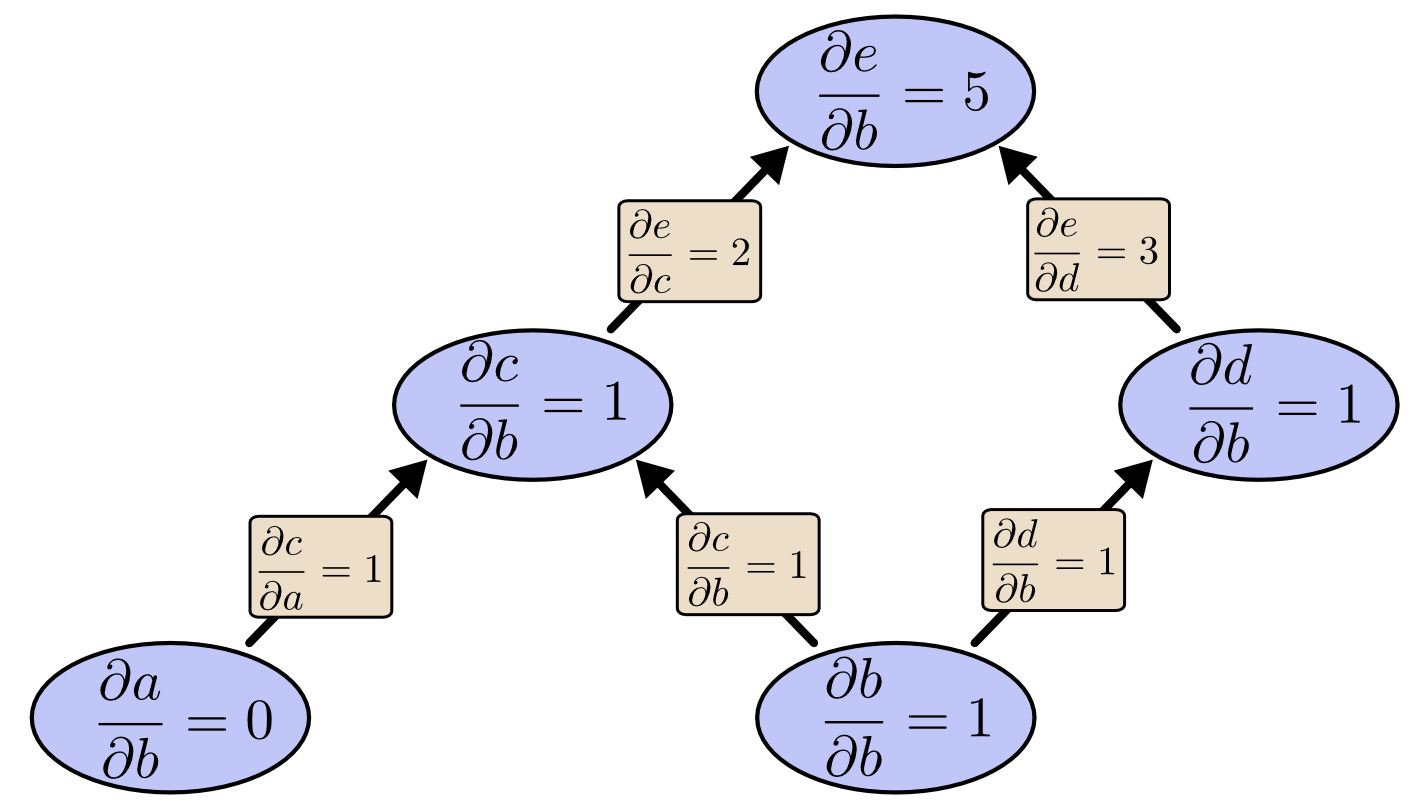
\includegraphics[width=\textwidth]{tree-forwardmode}
\caption{Вычисление произодной графа \cite{colah}.}
\end{figure}

Наиболее популярные системы, в которых реализовано автоматическое
дифференцирование: TensorFlow \cite{tf}, Theano \cite{theano},
Torch\cite{torch}. Существует большое число других систем и средств. В данной
работе используется система TensorFlow.

\subsection{Программные аспекты реализации вычислений}

В данной работе используется библиотека для глубинного машинного обучения и
система компьютерной алгебры TensorFlow. В этой системе всякая вычислительная
программа является ориентированным (вычислительным) графом, в котором вершины
являются операциями или данными, а ребра указывают направления <<движения>>
данных. Основной структурой данных является Tensor --- обобщение скаляров,
векторов-столбцов, строк, квадратных и прямоугольных матриц и вообще любого
многомерного массива. Отсюда и название системы <<TensorFlow>> --- <<поток
тензоров>>.

Программу, использующую TensorFlow, в простейшем случае можно условно разделить
на две части: в первой части определяется вычислительный граф, во второй части
этот граф запускается, исполняется. Создание графа --- процесс относительно
медленный и занимает единицы, а может и десятки секунд, этот процесс можно
сравнить с компиляцией. Зато по успешному завершению созданию графа получаем
быструю, эффективную, параллельную вычислительную программу, которая в
подавляющем большинстве случаев будет превосходить по скорости программы,
написанные за некоторое короткое время с нуля на языке C/С++.

Система TensorFlow использует результаты теории графов и позволяет эффективно 
распараллеливать алгоритмы. К тому же в системе заложен функционал, позволяющий
производить вычисления распределенно, на нескольких машинах.

\newpage
\section[Результаты экспериментальных модельных исследований]
{Результаты экспериментальных модельных \\исследований} 

\subsection{Пример 1}

Рассмотрим следующую модель.

\[
	\frac{d}{dt}\vec{x}(t) =
		\begin{pmatrix}
			-\theta_1 & 0 \\
			0 & -\theta_2
		\end{pmatrix}
		\vec{x}(t) 
		+
		\begin{pmatrix}
			1 & 0 \\
			0 & 1
		\end{pmatrix}
		\vec{u}(t) 
		+
		\begin{pmatrix}
			1 & 0 \\
			0 & 1
		\end{pmatrix}
		\vec{w}(t),
\]
\[
	\vec{y}(t_k) =
	\begin{pmatrix}
		1 & 0 \\
		0 & 1
	\end{pmatrix}
	\vec{x}(t_k) 
	+ 
	\vec{v}(t_k),
\]
\[
	\vec{x}(t) = \begin{bmatrix} x_1(t) \\ x_2(t) \end{bmatrix},\ 
	\vec{u}(t) = \begin{bmatrix} u_1(t) \\ u_2(t) \end{bmatrix},\
	\vec{w}(t) = \begin{bmatrix} w_1(t) \\ w_2(t) \end{bmatrix},\
	\vec{y}(t_k) = \begin{bmatrix} y_1(t_k) \\ y_2(t_k) \end{bmatrix},\
\]
\[
	\vec{v}(t_k) = \begin{bmatrix} v_1(t_k) \\ v_2(t_k) \end{bmatrix},\
\]
\[
	R = Q = P_0 = \begin{pmatrix} 0.01 & 0 \\ 0 & 0.01 \end{pmatrix},\
		\overline{\vec{x}_0} = \begin{pmatrix} 0 \\ 0 \end{pmatrix}
\]

$\theta = \begin{pmatrix} \theta_1 & \theta_2 \end{pmatrix}$ --- вектор
	оцениваемых параметров. \\ 
\indent $\theta^{*} = \begin{pmatrix} 1.0 & 1.0 \end{pmatrix}$ --- истинные
	значения параметров. \\
\indent Число параметров $s = 2$.

Входное воздействие --- ступенчатая функция
\[
	\vec{u}(t) = \begin{cases} \begin{pmatrix} 10 & 10 \end{pmatrix}^T,\ t > 0 \\
		\begin{pmatrix} 0 & 0 \end{pmatrix}^T,\ t = 0 \end{cases}
\]

% imports
\begin{pythontexcustomcode}{py}
import dill as pickle
from model.model import Model
import numpy as np
import pylatex
\end{pythontexcustomcode}

\renewcommand{\baselinestretch}{1}

% model definition and creation
\begin{pycode}[model]
F = lambda th: [[-th[0], 0.],
                [0., -th[1]]]

C = lambda th: [[1.0, 0.],
                [0., 1.0]]

G = lambda th: [[1.0, 0.],
                [0., 1.0]]

H = lambda th: [[1.0, 0.],
                [0., 1.0]]

x0_m = lambda th: [[0.],
                   [0.]]

x0_c = lambda th: [[1e-2, 0.],
                   [0., 1e-2]]
w_c = x0_c
v_c = x0_c

th = [1.0, 1.00]

m = Model(F, C, G, H, x0_m, x0_c, w_c, v_c, th)
\end{pycode}

% define input
\begin{pycode}[model]
t = np.linspace(0, 10, 100)
u = np.ones([2, 100])
u = u * 10

# run simulation
rez = m.sim(u, t)
y = rez[1]
\end{pycode}

Проведем процедуру оценивания параметров по одноточечному плану по
смоделированному отклику из некоторого начального приближения по параметрам.

% fit model and dump results to file
\begin{pycode}[model]
th0 = [0.8, 1.2]

fit = m.mle_fit(th0, t, u, y)

yhat_true = m.yhat(t, u, y)
yhat_est = m.yhat(t, u, y, fit.x)
init_loss = m.lik(t, u, y, th0)

rez = {'th0': th0, 'fit': fit, 'th_true': th, 'yhat_true': yhat_true,
	'yhat_est': yhat_est, 't': t, 'init_loss': init_loss}

filename = 'rez.pkl'
with open(filename, 'wb') as f:
	# pytex.add_created(filename)
	pickle.dump(rez, f)
\end{pycode}

% read fit results
\begin{pycode}
filename = 'rez.pkl'
pytex.add_dependencies(filename)

with open(filename, 'rb') as f:
	rez = pickle.load(f)

th0 = np.matrix(rez['th0'])
th0 = pylatex.Matrix(th0, mtype='b')
th0 = th0.dumps()

th = rez['fit']['x']
th = np.matrix(th)
th = np.around(th, 6)
th = pylatex.Matrix(th, mtype='b')
th = th.dumps()

fit = rez['fit']

th_true = rez['th_true']
th_t = np.matrix(th_true)
th_t = pylatex.Matrix(th_t, mtype='b')
th_t = th_t.dumps()

init_loss = rez['init_loss']
\end{pycode}

\bigskip \noindent
Истинные значения параметров 
\[
	\theta^{*} = \pyc{print(th_t)}
\]
Начальное приближение 
\[
	\theta_{0} = \pyc{print(th0)}
\]
Начальное значение критерия
\[
	\chi(\theta_0) = \pyc{print("%.6f" % init_loss)}
\]
Найденные значения параметров
\[
	\hat{\theta} = \pyc{print(th)}
\]
Значение критерия
\[
	\chi(\hat{\theta}) = \pyc{print("%.6f" % fit.fun)}
\]

Относительная погрешность оценивания в пространстве параметров

% compute fit relative tolerance
\begin{pycode}
th = rez['fit']['x']
th_t = rez['th_true']
rtol = np.linalg.norm(th_t - th) / np.linalg.norm(th_t)
rtol_p = "%.3f" % (rtol * 100)
\end{pycode}

\[
	\frac{||\theta^* -\ \hat{\theta}||}{||\theta^*||} = 
		\pyc{print("%.6f" % rtol)}
\]

% prepare relative tolerance in response space for display
\begin{pycode}
yhat_true = rez['yhat_true']
yhat_est = rez['yhat_est']

rtoly = np.linalg.norm(yhat_true - yhat_est)
rtolyp = "%.3f" % (rtoly * 100)
\end{pycode}

Относительная погрешность оценивания в пространстве откликов

\[
	\frac{||y^{*} -\ \hat{y}||}{|| y^{*} ||} = \pyc{print("%.6f" % rtoly)}
\]

\subsection{Пример 2}

Рассмотрим следующую модель.

\[
	\frac{d}{dt}\vec{x}(t) =
		\begin{pmatrix}
			-1 & 0 \\
			0 & -1
		\end{pmatrix}
		\vec{x}(t) 
		+
		\begin{pmatrix}
			\theta_1 & 0 \\
			0 & \theta_2 
		\end{pmatrix}
		\vec{u}(t) 
		+
		\begin{pmatrix}
			1 & 0 \\
			0 & 1
		\end{pmatrix}
		\vec{w}(t),
\]
\[
	\vec{y}(t_k) =
	\begin{pmatrix}
		1 & 0 \\
		0 & 1
	\end{pmatrix}
	\vec{x}(t_k) 
	+ 
	\vec{v}(t_k),
\]
\[
	\vec{x}(t) = \begin{bmatrix} x_1(t) \\ x_2(t) \end{bmatrix},\ 
	\vec{u}(t) = \begin{bmatrix} u_1(t) \\ u_2(t) \end{bmatrix},\
	\vec{w}(t) = \begin{bmatrix} w_1(t) \\ w_2(t) \end{bmatrix},\
	\vec{y}(t_k) = \begin{bmatrix} y_1(t_k) \\ y_2(t_k) \end{bmatrix},\
\]
\[
	\vec{v}(t_k) = \begin{bmatrix} v_1(t_k) \\ v_2(t_k) \end{bmatrix},\
\]
\[
	R = Q = P_0 = \begin{pmatrix} 0.01 & 0 \\ 0 & 0.01 \end{pmatrix},\
		\overline{\vec{x}_0} = \begin{pmatrix} 0 \\ 0 \end{pmatrix}
\]

$\theta = \begin{pmatrix} \theta_1 & \theta_2 \end{pmatrix}$ --- вектор
	оцениваемых параметров. \\ 
\indent $\theta^{*} = \begin{pmatrix} 1.0 & 1.0 \end{pmatrix}$ --- истинные
	значения параметров. \\
\indent Число параметров $s = 2$.

Входное воздействие --- ступенчатая функция
\[
	\vec{u}(t) = \begin{cases} \begin{pmatrix} 10 & 10 \end{pmatrix}^T,\ t > 0 \\
		\begin{pmatrix} 0 & 0 \end{pmatrix}^T,\ t = 0 \end{cases}
\]

% define create model
\begin{pycode}[model2]
F = lambda th: [[-1, 0.],
								[0., -1]]

C = lambda th: [[th[0], 0.],
								[0., th[1]]]

G = lambda th: [[1.0, 0.],
                [0., 1.0]]

H = lambda th: [[1.0, 0.],
                [0., 1.0]]

x0_m = lambda th: [[0.],
                   [0.]]

x0_c = lambda th: [[1e-2, 0.],
                   [0., 1e-2]]
w_c = x0_c
v_c = x0_c

th = [1.0, 1.00]

m = Model(F, C, G, H, x0_m, x0_c, w_c, v_c, th)
\end{pycode}

% define input
\begin{pycode}[model2]
t = np.linspace(0, 10, 100)
u = np.ones([2, 100])
u = u * 10

# run simulation
rez = m.sim(u, t)
y = rez[1]
\end{pycode}

% fit model and dump results to file
\begin{pycode}[model2]
th0 = [0.8, 1.2]

fit = m.mle_fit(th0, t, u, y)

yhat_true = m.yhat(t, u, y)
yhat_est = m.yhat(t, u, y, fit.x)
init_loss = m.lik(t, u, y, th0)

rez = {'th0': th0, 'fit': fit, 'th_true': th, 'yhat_true': yhat_true,
	'yhat_est': yhat_est, 't': t, 'init_loss': init_loss}

filename = 'rez2.pkl'
with open(filename, 'wb') as f:
	# pytex.add_created(filename)
	pickle.dump(rez, f)
\end{pycode}

% read fit results
\begin{pycode}
filename = 'rez2.pkl'
pytex.add_dependencies(filename)

with open(filename, 'rb') as f:
	rez = pickle.load(f)

th0 = np.matrix(rez['th0'])
th0 = pylatex.Matrix(th0, mtype='b')
th0 = th0.dumps()

th = rez['fit']['x']
th = np.matrix(th)
th = np.around(th, 6)
th = pylatex.Matrix(th, mtype='b')
th = th.dumps()

fit = rez['fit']

th_true = rez['th_true']
th_t = np.matrix(th_true)
th_t = pylatex.Matrix(th_t, mtype='b')
th_t = th_t.dumps()

init_loss = rez['init_loss']
\end{pycode}

\bigskip \noindent
Истинные значения параметров 
\[
	\theta^{*} = \pyc{print(th_t)}
\]
Начальное приближение 
\[
	\theta_{0} = \pyc{print(th0)}
\]
Начальное значение критерия
\[
	\chi(\theta_0) = \pyc{print("%.6f" % init_loss)}
\]
Найденные значения параметров
\[
	\hat{\theta} = \pyc{print(th)}
\]
Значение критерия
\[
	\chi(\hat{\theta}) = \pyc{print("%.6f" % fit.fun)}
\]

Относительная погрешность оценивания в пространстве параметров

% compute fit relative tolerance
\begin{pycode}
th = rez['fit']['x']
th_t = rez['th_true']
rtol = np.linalg.norm(th_t - th) / np.linalg.norm(th_t)
rtol_p = "%.3f" % (rtol * 100)
\end{pycode}

\[
	\frac{||\theta^* -\ \hat{\theta}||}{||\theta^*||} = 
		\pyc{print("%.6f" % rtol)}
\]

% prepare relative tolerance in response space for display
\begin{pycode}
yhat_true = rez['yhat_true']
yhat_est = rez['yhat_est']

rtoly = np.linalg.norm(yhat_true - yhat_est)
rtolyp = "%.3f" % (rtoly * 100)
\end{pycode}

Относительная погрешность оценивания в пространстве откликов

\[
	\frac{||y^{*} -\ \hat{y}||}{|| y^{*} ||} = \pyc{print("%.6f" % rtoly)}
\]

\subsection{Пример 3}

Рассмотрим следующую модель.

\[
	\frac{d}{dt}\vec{x}(t) =
		\begin{pmatrix}
			-1 & 0 \\
			0 & -1
		\end{pmatrix}
		\vec{x}(t) 
		+
		\begin{pmatrix}
			1 & 0 \\
			0 & 1 
		\end{pmatrix}
		\vec{u}(t) 
		+
		\begin{pmatrix}
			\theta_1 & 0 \\
			0 & \theta_2
		\end{pmatrix}
		\vec{w}(t),
\]
\[
	\vec{y}(t_k) =
	\begin{pmatrix}
		1 & 0 \\
		0 & 1
	\end{pmatrix}
	\vec{x}(t_k) 
	+ 
	\vec{v}(t_k),
\]
\[
	\vec{x}(t) = \begin{bmatrix} x_1(t) \\ x_2(t) \end{bmatrix},\ 
	\vec{u}(t) = \begin{bmatrix} u_1(t) \\ u_2(t) \end{bmatrix},\
	\vec{w}(t) = \begin{bmatrix} w_1(t) \\ w_2(t) \end{bmatrix},\
	\vec{y}(t_k) = \begin{bmatrix} y_1(t_k) \\ y_2(t_k) \end{bmatrix},\
\]
\[
	\vec{v}(t_k) = \begin{bmatrix} v_1(t_k) \\ v_2(t_k) \end{bmatrix},\
\]
\[
	R = Q = P_0 = \begin{pmatrix} 0.01 & 0 \\ 0 & 0.01 \end{pmatrix},\
		\overline{\vec{x}_0} = \begin{pmatrix} 0 \\ 0 \end{pmatrix}
\]

$\theta = \begin{pmatrix} \theta_1 & \theta_2 \end{pmatrix}$ --- вектор
	оцениваемых параметров. \\ 
\indent $\theta^{*} = \begin{pmatrix} 1.0 & 1.0 \end{pmatrix}$ --- истинные
	значения параметров. \\
\indent Число параметров $s = 2$.

Входное воздействие --- ступенчатая функция
\[
	\vec{u}(t) = \begin{cases} \begin{pmatrix} 10 & 10 \end{pmatrix}^T,\ t > 0 \\
		\begin{pmatrix} 0 & 0 \end{pmatrix}^T,\ t = 0 \end{cases}
\]

% define create model
\begin{pycode}[model3]
F = lambda th: [[-1, 0.],
                [0., -1]]

C = lambda th: [[1, 0.],
                [0., 1]]

G = lambda th: [[th[0], 0.],
                [0., th[1]]]

H = lambda th: [[1.0, 0.],
                [0., 1.0]]

x0_m = lambda th: [[0.],
                   [0.]]

x0_c = lambda th: [[1e-2, 0.],
                   [0., 1e-2]]
w_c = x0_c
v_c = x0_c

th = [1.0, 1.00]

m = Model(F, C, G, H, x0_m, x0_c, w_c, v_c, th)
\end{pycode}

% define input
\begin{pycode}[model3]
t = np.linspace(0, 10, 100)
u = np.ones([2, 100])
u = u * 10

# run simulation
rez = m.sim(u, t)
y = rez[1]
\end{pycode}

% fit model and dump results to file
\begin{pycode}[model3]
th0 = [0.8, 1.2]

fit = m.mle_fit(th0, t, u, y)

yhat_true = m.yhat(t, u, y)
yhat_est = m.yhat(t, u, y, fit.x)
init_loss = m.lik(t, u, y, th0)

rez = {'th0': th0, 'fit': fit, 'th_true': th, 'yhat_true': yhat_true,
	'yhat_est': yhat_est, 't': t, 'init_loss': init_loss}

filename = 'rez3.pkl'
with open(filename, 'wb') as f:
	# pytex.add_created(filename)
	pickle.dump(rez, f)
\end{pycode}

% read fit results
\begin{pycode}
filename = 'rez3.pkl'
pytex.add_dependencies(filename)

with open(filename, 'rb') as f:
	rez = pickle.load(f)

th0 = np.matrix(rez['th0'])
th0 = pylatex.Matrix(th0, mtype='b')
th0 = th0.dumps()

th = rez['fit']['x']
th = np.matrix(th)
th = np.around(th, 6)
th = pylatex.Matrix(th, mtype='b')
th = th.dumps()

fit = rez['fit']

th_true = rez['th_true']
th_t = np.matrix(th_true)
th_t = pylatex.Matrix(th_t, mtype='b')
th_t = th_t.dumps()

init_loss = rez['init_loss']
\end{pycode}

\bigskip \noindent
Истинные значения параметров 
\[
	\theta^{*} = \pyc{print(th_t)}
\]
Начальное приближение 
\[
	\theta_{0} = \pyc{print(th0)}
\]
Начальное значение критерия
\[
	\chi(\theta_0) = \pyc{print("%.6f" % init_loss)}
\]
Найденные значения параметров
\[
	\hat{\theta} = \pyc{print(th)}
\]
Значение критерия
\[
	\chi(\hat{\theta}) = \pyc{print("%.6f" % fit.fun)}
\]

Относительная погрешность оценивания в пространстве параметров

% compute fit relative tolerance
\begin{pycode}
th = rez['fit']['x']
th_t = rez['th_true']
rtol = np.linalg.norm(th_t - th) / np.linalg.norm(th_t)
rtol_p = "%.3f" % (rtol * 100)
\end{pycode}

\[
	\frac{||\theta^* -\ \hat{\theta}||}{||\theta^*||} = 
		\pyc{print("%.6f" % rtol)}
\]

% prepare relative tolerance in response space for display
\begin{pycode}
yhat_true = rez['yhat_true']
yhat_est = rez['yhat_est']

rtoly = np.linalg.norm(yhat_true - yhat_est)
rtolyp = "%.3f" % (rtoly * 100)
\end{pycode}

Относительная погрешность оценивания в пространстве откликов

\[
	\frac{||y^{*} -\ \hat{y}||}{|| y^{*} ||} = \pyc{print("%.6f" % rtoly)}
\]

В данном примере в результатах наблюдается крайне высокий уровень погрешности в
  силу того, что оцениваются параметры матрицы $G$ --- матрицы влияния
  возмущений объекта на его состояние. Параметры, входящие в эту матрицу плохо
  поддаются оценке. Возможная мера, которую можно принять для улучшения оценок,
  является оценивание с использованием предварительно синтезированных
  оптимальных входных сигналах, то есть предварительное планирование входных
  сигналов.

\subsection{Пример 4}

Рассмотрим следующую модель.

\[
	\frac{d}{dt}\vec{x}(t) =
		\begin{pmatrix}
			-1 & 0 \\
			0 & -1
		\end{pmatrix}
		\vec{x}(t) 
		+
		\begin{pmatrix}
			1 & 0 \\
			0 & 1 
		\end{pmatrix}
		\vec{u}(t) 
		+
		\begin{pmatrix}
			1 & 0 \\
			0 & 1 
		\end{pmatrix}
		\vec{w}(t),
\]
\[
	\vec{y}(t_k) =
	\begin{pmatrix}
		\theta_1 & 0 \\
		0 & \theta_2
	\end{pmatrix}
	\vec{x}(t_k) 
	+ 
	\vec{v}(t_k),
\]
\[
	\vec{x}(t) = \begin{bmatrix} x_1(t) \\ x_2(t) \end{bmatrix},\ 
	\vec{u}(t) = \begin{bmatrix} u_1(t) \\ u_2(t) \end{bmatrix},\
	\vec{w}(t) = \begin{bmatrix} w_1(t) \\ w_2(t) \end{bmatrix},\
	\vec{y}(t_k) = \begin{bmatrix} y_1(t_k) \\ y_2(t_k) \end{bmatrix},\
\]
\[
	\vec{v}(t_k) = \begin{bmatrix} v_1(t_k) \\ v_2(t_k) \end{bmatrix},\
\]
\[
	R = Q = P_0 = \begin{pmatrix} 0.01 & 0 \\ 0 & 0.01 \end{pmatrix},\
		\overline{\vec{x}_0} = \begin{pmatrix} 0 \\ 0 \end{pmatrix}
\]

$\theta = \begin{pmatrix} \theta_1 & \theta_2 \end{pmatrix}$ --- вектор
	оцениваемых параметров. \\ 
\indent $\theta^{*} = \begin{pmatrix} 1.0 & 1.0 \end{pmatrix}$ --- истинные
	значения параметров. \\
\indent Число параметров $s = 2$.

Входное воздействие --- ступенчатая функция
\[
	\vec{u}(t) = \begin{cases} \begin{pmatrix} 10 & 10 \end{pmatrix}^T,\ t > 0 \\
		\begin{pmatrix} 0 & 0 \end{pmatrix}^T,\ t = 0 \end{cases}
\]

% define create model
\begin{pycode}[model4]
F = lambda th: [[-1, 0.],
                [0., -1]]

C = lambda th: [[1, 0.],
                [0., 1]]

G = lambda th: [[1, 0.],
                [0., 1]]

H = lambda th: [[th[0], 0.],
                [0., th[1]]]

x0_m = lambda th: [[0.],
                   [0.]]

x0_c = lambda th: [[1e-2, 0.],
                   [0., 1e-2]]
w_c = x0_c
v_c = x0_c

th = [1.0, 1.0]

m = Model(F, C, G, H, x0_m, x0_c, w_c, v_c, th)
\end{pycode}

% define input
\begin{pycode}[model4]
t = np.linspace(0, 10, 100)
u = np.ones([2, 100])
u = u * 10

# run simulation
rez = m.sim(u, t)
y = rez[1]
\end{pycode}

% fit model and dump results to file
\begin{pycode}[model4]
th0 = [0.9, 1.1] 


fit = m.mle_fit(th0, t, u, y)

yhat_true = m.yhat(t, u, y)
yhat_est = m.yhat(t, u, y, fit.x)
init_loss = m.lik(t, u, y, th0)

rez = {'th0': th0, 'fit': fit, 'th_true': th, 'yhat_true': yhat_true,
	'yhat_est': yhat_est, 't': t, 'init_loss': init_loss}

filename = 'rez4.pkl'
with open(filename, 'wb') as f:
	# pytex.add_created(filename)
	pickle.dump(rez, f)
\end{pycode}

% read fit results
\begin{pycode}
filename = 'rez4.pkl'
pytex.add_dependencies(filename)
 
with open(filename, 'rb') as f:
	rez = pickle.load(f)

th0 = np.matrix(rez['th0'])
th0 = pylatex.Matrix(th0, mtype='b')
th0 = th0.dumps()

th = rez['fit']['x']
th = np.matrix(th)
th = np.around(th, 6)
th = pylatex.Matrix(th, mtype='b')
th = th.dumps()

fit = rez['fit']

th_true = rez['th_true']
th_t = np.matrix(th_true)
th_t = pylatex.Matrix(th_t, mtype='b')
th_t = th_t.dumps()

init_loss = rez['init_loss']
\end{pycode}

\bigskip \noindent
Истинные значения параметров 
\[
	\theta^{*} = \pyc{print(th_t)}
\]
Начальное приближение 
\[
	\theta_{0} = \pyc{print(th0)}
\]
Начальное значение критерия
\[
	\chi(\theta_0) = \pyc{print("%.6f" % init_loss)}
\]
Найденные значения параметров
\[
	\hat{\theta} = \pyc{print(th)}
\]
Значение критерия
\[
	\chi(\hat{\theta}) = \pyc{print("%.6f" % fit.fun)}
\]

Относительная погрешность оценивания в пространстве параметров

% compute fit relative tolerance
\begin{pycode}
th = rez['fit']['x']
th_t = rez['th_true']
rtol = np.linalg.norm(th_t - th) / np.linalg.norm(th_t)
rtol_p = "%.3f" % (rtol * 100)
\end{pycode}

\[
	\frac{||\theta^* -\ \hat{\theta}||}{||\theta^*||} = 
		\pyc{print("%.6f" % rtol)}
\]

% prepare relative tolerance in response space for display
\begin{pycode}
yhat_true = rez['yhat_true']
yhat_est = rez['yhat_est']

rtoly = np.linalg.norm(yhat_true - yhat_est)
rtolyp = "%.3f" % (rtoly * 100)
\end{pycode}

Относительная погрешность оценивания в пространстве откликов

\[
	\frac{||y^{*} -\ \hat{y}||}{|| y^{*} ||} = \pyc{print("%.6f" % rtoly)}
\]

\subsection{Пример 5}

Рассмотрим следующую модель.

\[
	\frac{d}{dt}\vec{x}(t) =
		\begin{pmatrix}
			-1 & 0 \\
			0 & -1
		\end{pmatrix}
		\vec{x}(t) 
		+
		\begin{pmatrix}
			1 & 0 \\
			0 & 1 
		\end{pmatrix}
		\vec{u}(t) 
		+
		\begin{pmatrix}
			1 & 0 \\
			0 & 1 
		\end{pmatrix}
		\vec{w}(t),
\]
\[
	\vec{y}(t_k) =
	\begin{pmatrix}
		1 & 0 \\
		0 & 1
	\end{pmatrix}
	\vec{x}(t_k) 
	+ 
	\vec{v}(t_k),
\]
\[
	\vec{x}(t) = \begin{bmatrix} x_1(t) \\ x_2(t) \end{bmatrix},\ 
	\vec{u}(t) = \begin{bmatrix} u_1(t) \\ u_2(t) \end{bmatrix},\
	\vec{w}(t) = \begin{bmatrix} w_1(t) \\ w_2(t) \end{bmatrix},\
	\vec{y}(t_k) = \begin{bmatrix} y_1(t_k) \\ y_2(t_k) \end{bmatrix},\
\]
\[
	\vec{v}(t_k) = \begin{bmatrix} v_1(t_k) \\ v_2(t_k) \end{bmatrix},\
\]
\[
	R = P_0 = \begin{pmatrix} 0.01 & 0 \\ 0 & 0.01 \end{pmatrix},\
		\overline{\vec{x}_0} = \begin{pmatrix} 0 \\ 0 \end{pmatrix},\ Q =
      \begin{pmatrix} \theta_1 & 0 \\ 0 & \theta_2 \end{pmatrix}
\]

$\theta = \begin{pmatrix} \theta_1 & \theta_2 \end{pmatrix}$ --- вектор
	оцениваемых параметров. \\ 
\indent $\theta^{*} = \begin{pmatrix} 1.0 & 1.0 \end{pmatrix}$ --- истинные
	значения параметров. \\
\indent Число параметров $s = 2$.

Входное воздействие --- ступенчатая функция
\[
	\vec{u}(t) = \begin{cases} \begin{pmatrix} 10 & 10 \end{pmatrix}^T,\ t > 0 \\
		\begin{pmatrix} 0 & 0 \end{pmatrix}^T,\ t = 0 \end{cases}
\]

% define create model
\begin{pycode}[model5]
F = lambda th: [[-1, 0.],
                [0., -1]]

C = lambda th: [[1, 0.],
                [0., 1]]

G = lambda th: [[1, 0.],
                [0., 1]]

H = lambda th: [[1, 0.],
                [0., 1]]

x0_m = lambda th: [[0.],
                   [0.]]

x0_c = lambda th: [[1e-2, 0.],
                   [0., 1e-2]]

w_c = lambda th: [[th[0], 0],
                  [0, th[1]]]
v_c = x0_c

th = [0.1, 0.1]

m = Model(F, C, G, H, x0_m, x0_c, w_c, v_c, th)
\end{pycode}

% define input
\begin{pycode}[model5]
t = np.linspace(0, 10, 100)
u = np.ones([2, 100])
u = u * 10

# run simulation
rez = m.sim(u, t)
y = rez[1]
\end{pycode}

% fit model and dump results to file
\begin{pycode}[model5]
th0 = [0.11, 0.09] 


fit = m.mle_fit(th0, t, u, y)

yhat_true = m.yhat(t, u, y)
yhat_est = m.yhat(t, u, y, fit.x)
init_loss = m.lik(t, u, y, th0)

rez = {'th0': th0, 'fit': fit, 'th_true': th, 'yhat_true': yhat_true,
	'yhat_est': yhat_est, 't': t, 'init_loss': init_loss}

filename = 'rez5.pkl'
with open(filename, 'wb') as f:
	# pytex.add_created(filename)
	pickle.dump(rez, f)
\end{pycode}

% read fit results
\begin{pycode}
filename = 'rez5.pkl'
pytex.add_dependencies(filename)
 
with open(filename, 'rb') as f:
	rez = pickle.load(f)

th0 = np.matrix(rez['th0'])
th0 = pylatex.Matrix(th0, mtype='b')
th0 = th0.dumps()

th = rez['fit']['x']
th = np.matrix(th)
th = np.around(th, 6)
th = pylatex.Matrix(th, mtype='b')
th = th.dumps()

fit = rez['fit']

th_true = rez['th_true']
th_t = np.matrix(th_true)
th_t = pylatex.Matrix(th_t, mtype='b')
th_t = th_t.dumps()

init_loss = rez['init_loss']
\end{pycode}

\bigskip \noindent
Истинные значения параметров 
\[
	\theta^{*} = \pyc{print(th_t)}
\]
Начальное приближение 
\[
	\theta_{0} = \pyc{print(th0)}
\]
Начальное значение критерия
\[
	\chi(\theta_0) = \pyc{print("%.6f" % init_loss)}
\]
Найденные значения параметров
\[
	\hat{\theta} = \pyc{print(th)}
\]
Значение критерия
\[
	\chi(\hat{\theta}) = \pyc{print("%.6f" % fit.fun)}
\]

Относительная погрешность оценивания в пространстве параметров

% compute fit relative tolerance
\begin{pycode}
th = rez['fit']['x']
th_t = rez['th_true']
rtol = np.linalg.norm(th_t - th) / np.linalg.norm(th_t)
rtol_p = "%.3f" % (rtol * 100)
\end{pycode}

\[
	\frac{||\theta^* -\ \hat{\theta}||}{||\theta^*||} = 
		\pyc{print("%.6f" % rtol)}
\]

% prepare relative tolerance in response space for display
\begin{pycode}
yhat_true = rez['yhat_true']
yhat_est = rez['yhat_est']

rtoly = np.linalg.norm(yhat_true - yhat_est)
rtolyp = "%.3f" % (rtoly * 100)
\end{pycode}

Относительная погрешность оценивания в пространстве откликов

\[
	\frac{||y^{*} -\ \hat{y}||}{|| y^{*} ||} = \pyc{print("%.6f" % rtoly)}
\]

\section*{Заключение}
\addcontentsline{toc}{section}{Заключение}

Как было показано, результаты экспериментальных модельных исследований хорошо
согласуются с теоретическими положениями об эффективности алгоритма оценивания
параметров динамических стохастических линейных \allowbreak
\mbox{непрерывно-дискретных} систем методом максимального правдоподобия при
выполнении соответствующих
указанных априорных предположений. 

А использование в оптимизационной процедуре градиента,
вычисленного методом автоматического дифференцирования, позволяет получить
оценки, погрешность которых сопоставима с погрешностью оценок, полученных с
использованием аналитического выражения градиента.

\begin{thebibliography}{9}

\begin{hyphenrules}{nohyphenation} 

% FIXME: fix to conform with GOST

\begin{sloppypar}

\bibitem{denisov} Активная параметрическая идентификация стохастических
линейных систем: монография / В.И. Денисов, В.М. Чубич, О.С. Черникова, Д.И.
	Бобылева. --- Новосибирск : Изд-во НГТУ, 2009. --- 192 с.
	\mbox{(Серия <<Монографии НГТУ>>)}.

\bibitem{chubich} Активная параметрическая идентификация стохастических
	динамических систем. Оценивание параметров: учеб. пособие / В.М. Чубич,
	\mbox{Е.В. Филиппова}. --- Новосибирск: Изд-во НГТУ, 2016. --- 63 с.

\bibitem{colah} Chris Olah. ''Calculus on Computational Graphs:
Backpropagation'', colah's blog. August 31, 2015.
URL: colah.github.io/posts/2015-08-Backprop

\bibitem{ad-ml-survey} A. Baydin, B. Pearlmutter, A. Radul, J. Siskind.
Automatic Differentiation in Machine Learning: a Survey. {arXiv:0706.1234 [cs.SC]}

% плохое оформление библиографии или плохой источник?
\bibitem{tf} Martín Abadi, Ashish Agarwal, Paul Barham, et al.
TensorFlow: Large-scale machine learning on heterogeneous systems,
2015. Software available from tensorflow.org. {arXiv:1603.04467 [cs.DC]}

\bibitem{theano} J. Bergstra, O. Breuleux, F. Bastien, et al. “Theano: A CPU
and GPU Math Expression Compiler”. Proceedings of the Python for Scientific
Computing Conference (SciPy) 2010. June 30 - July 3, Austin, TX

\bibitem{torch} Collobert, Ronan, Koray Kavukcuoglu, and Clément Farabet.
"Torch7: A matlab-like environment for machine learning." BigLearn, NIPS
Workshop. No. EPFL-CONF-192376. 2011.

\end{sloppypar}

\end{hyphenrules}

\end{thebibliography}

\end{document}


blogposts:
==========

justin domke associate professor, 2009, college of computing and information
sciences, university of massachusetts,
automatic-differentiation-the-most-criminally-underused-tool-in-the-potential
machine-learning-toolbox/


articles:
=========


# vim: ts=2 sw=2
